%-----------------------------------------------------------------------------
%
%               Template for sigplanconf LaTeX Class
%
% Name:         sigplanconf-template.tex
%
% Purpose:      A template for sigplanconf.cls, which is a LaTeX 2e class
%               file for SIGPLAN conference proceedings.
%
% Author:       Paul C. Anagnostopoulos
%               Windfall Software
%               978 371-2316
%               paul@windfall.com
%
% Created:      15 February 2005
%
%-----------------------------------------------------------------------------


\documentclass[]{sigplanconf}

% The following \documentclass options may be useful:
%
% 10pt          To set in 10-point type instead of 9-point.
% 11pt          To set in 11-point type instead of 9-point.
% authoryear    To obtain author/year citation style instead of numeric.

\usepackage{amsmath}
\usepackage{graphicx}
\usepackage{url}
\usepackage{amssymb}
\usepackage{subfigure}
\usepackage{algorithm} 
\usepackage{algpseudocode}



% make an environment for subfigures with verbatim
\newbox\subfigbox	% Create a box to hold the subfigure. 
\makeatletter
  \newenvironment{subfloat}% % Create the new environment. 
    {\def\caption##1{\gdef\subcapsave{\relax##1}}%
    \let\subcapsave=\@empty % Save the subcaption text.  
    \let\sf@oldlabel=\label 
    \def\label##1{\xdef\sublabsave{\noexpand\label{##1}}}%
    \let\sublabsave\relax  %
    \setbox\subfigbox\hbox 
        \bgroup}% 
     {\egroup   %
    \let\label=\sf@oldlabel
    \subfigure[\subcapsave]{\box\subfigbox}}% 
\makeatother

\newcommand{\eightpoint}{\fontsize{8pt}{10pt}\selectfont}
\newcommand{\ninepoint}{\fontsize{9pt}{11pt}\selectfont}


% do not indent paragraphs of enumerated lists (my lists go on for pages...)
% numbers flush left to paragraph text: \leftmargin=17pt
\newcommand{\mybegin}{\begin{list}{\labelenumi}{\leftmargin=\parindent}\usecounter{enumi}}
%\newcommand{\myitem}[1]{\item {\textit{\textbf{#1}}}}
\newcommand{\myitem}[1]{\item {\bf #1}}
\newcommand{\myend}{\end{list}}
\newcommand{\mt}[1]{\mbox{\it #1}}
\newcommand{\todo}[1]{\framebox {\bf #1}}



\begin{document}

\conferenceinfo{PLDI  2011}{June 2011, San Jose, CA.} 
\copyrightyear{2010} 
\copyrightdata{[to be supplied]} 

%\titlebanner{banner above paper title}        % These are ignored unless
%\preprintfooter{short description of paper}   % 'preprint' option specified.

\title{Sliding Window Computations in Stream Programs}
%\subtitle{Subtitle Text, if any}

\authorinfo{}
           {}
            {}
% \authorinfo{Name2\and Name3}
%            {Affiliation2/3}
%            {Email2/3}

\maketitle
\begin{abstract}
Applications that are structured around some notion of a "stream"
are becoming increasingly important and widespread.  There is
evidence that streaming media applications are already consuming
most of the cycles on consumer machines \cite{Rix98}, and their
use is continuing to grow.  {\StreamIt} is a language and compiler
specifically designed for modern stream programming.  Despite the
prevalence of these applications, there is surprisingly little
language and compiler for practical, large-scale stream
programming.  {\StreamIt} is a language and compiler specifically
designed for modern stream programming.  The {\StreamIt} langauge
holds two goals: first, to provide high-level stream abstractions
that improve programmer productivity and program robustness within
the streaming domain; second, to serve as a common machine
language for grid-based processors.  At the same time, {\StreamIt}
compiler aims to perform stream-specific optimizations to achieve
the performance of an expert programmer.  This thesis develops
several techniques for scheduling execution of {\filters} in
{\StreamIt}.  The work focuses on correctness as well as
minimizing buffering requirements and stored schedule size.

\end{abstract}

%\category{CR-number}{subcategory}{third-level}

%\terms
%term1, term2

%\keywords
%keyword1, keyword2

\section{Introduction}

The domain of stream programs is important because it stands at the
intersection of trends in applications and architectures.  Stream
programming naturally represents applications such as audio, video,
digital signal processing, and data analysis; applications that are
increasing prevalent as computing moves towards data-centric
applications and to the mobile and embedded space.  Also, by virtue of
their structure -- a graph of independent computational nodes (termed
{\it filters}) with explicit and regular communication -- stream
programs are a natural fit for exploiting coarse-grained parallelism
suitable for multicore architectures.  The interest in streaming
applications has spawned a number of streaming languages that target
the streaming domain, including StreamIt~\cite{streamitcc},
Brook~\cite{brook04}, Cg~\cite{cg03},
SPUR~\cite{spur05samos}, Spidle~\cite{spidle03}, Lime~\cite{lime10},
and SPL~\cite{spl09}.

In a stream program, filters define an atomic execution step that
repeats for many iterations; each execution step discards a number of
data items from filter's input edge.  Often, a filter does not discard
all the data items that it read for the current execution step,
requiring these inspected (but not discarded) items for a future
iteration (or iterations) of the filter.  This type of filter is
described as performing a sliding window computation on its
input. Sliding window computations are prevalent in stream programs.
Examples of sliding window computations include FIR filters; moving
averages and differences; error correcting codes; motion estimation;
and network packet inspection.  A recent study of a large streaming
benchmark suite written in the StreamIt programming language finds
that 17 of the 30 real-world benchmarks include at least one filter
that performs a sliding window computation~\cite{streamit-suite}.


Figure~\ref{fig:fir-nopeeking} shows how to perform a sliding
window FIR filter via state carried between iterations of a filter.
This implementation is difficult for the compiler to analyze and
reason about.  Some programming languages (e.g., Brook, Lime,
StreamIt, and IBM SPL) go so far as to include idioms that directly
represent sliding window computation, allowing the programmer to
specify, for each filter, the size of the window and the number of
items discarded after an execution of the filter.
Figure~\ref{fig:fir-peeking} shows how language extensions of the
StreamIt programming language elegantly expose sliding windows for
compiler analysis and optimization.

A goal of stream programming is to directly expose to the software
layer the necessary information to enable automatic management of
coarse-grained parallelism.  Stream programs expose multiple forms of
parallelism: pipeline parallelism that exists between producers and
consumers; task parallelism that exists between pairs of filters on
parallel branches of the stream graph; and data parallelism that
exists when a filter is stateless and can thus be replicated.  Data
parallelism is the most attractive, as it provides load-balanced and
limitless parallelism (as long as input data is available).  A filter
that is stateful, and cannot be data-parallelized, becomes a limit to
parallelization scalability, as the work of that filter cannot be
divided; the most load-intensive stateful filter becomes a
bottleneck.

This paper presents a compiler framework for data-parallelizing
filters that perform sliding window computations when the properties
of the sliding window can be calculated statically.  If sliding window
filters required state, this state would represent a new
parallelization bottleneck.  Sliding windows are the bottleneck in 11
of the 17 real-world benchmarks in the StreamIt Benchmark Suite that
contain sliding windows~\cite{streamit-suite}.  For example, examining
the Channelvocoder benchmark, this state would limit scalability to 18
cores, whereas our techniques scale to at least 64 cores.

Data-parallelizing a filter is performed via a transformation termed
{\it fission} (verb form {\it fiss})~\cite{streamit-asplos}.  Fission
is the process of data-parallelizing a stateless filter by duplicating
the filter a certain number of ways, assigning duplicates to distinct
cores, and correctly distributed input data to and collecting output
data from the duplicates.  The duplicated filters are referred to as
{\it products}.  When a sliding window is present, fission is
accomplished by duplicating certain input items since they are
required by multiple products.  This duplication translates into
inter-core communication, a limiting factor for scalability when
targeting multicore architectures.

Previous approaches duplicate each input data item to all products,
with products ignoring (decimating) items that are not
needed~\cite{streamit-asplos}.  We will show that this strategy limits
scalability for multicores by requiring too much inter-core
communication.  In contrast, our strategy precisely routes each input
item to the minimal set of product filters that requires the item.
Unlike previous work, our techniques are defined on
multiple input and multiple output filters, removing the need to
introduce synchronization filters that serialize data before and
after the product filters.  

Our techniques operate on {\it static-rate} stream graphs, meaning
that the number of items produced, the number of items consumed, and
the number of items inspected by each filter can be determined
statically.  Because of this property, a steady-state schedule of
filter firings can be calculated that does not grow buffers and can be
executed indefinitely~\cite{lee87}.  Our techniques are conscious of
the spatial locality between producers and consumers.  Our framework
includes techniques that can determine when spatial locality can be
increased by altering the steady-state schedule.  When applicable, our
techniques can reduce the overall sharing (and thus inter-core
communication) requirement to below a threshold percent of the total
input communication for each sliding window filter that is
data-parallelized. 

\begin{figure}[t]
\centering
\subfigure[]{\includegraphics[width=3.3in]{figures/fir-nopeeking.pdf}\label{fig:fir-nopeeking}}
\subfigure[]{\includegraphics[width=3.3in]{figures/fir-peeking.pdf}\label{fig:fir-peeking}}
\caption[Two implementations of an FIR filter.]{\label{fig:fir-code}
  Two StreamIt implementations of an FIR filter:
   (a) the non-peeking version implemented via a
  stateful circular buffer; and (b) the peeking version. Only steady-state implementation is
  given.}
\end{figure}

The framework presented is defined on a model of computation that is
agnostic of source language.  To evaluate our techniques we have
implemented them in the context of the StreamIt compiler
infrastructure~\cite{gordon-asplos06}.  Our transformations are guided
by the parallelization management techniques presented
in~\cite{gordon-asplos06}.  We employ 3 real-world benchmarks from the
StreamIt Benchmark Suite~\cite{streamit-suite} that include sliding
window computation.  We demonstrate the effectiveness of our
techniques by comparing them to previously published techniques on 2
multicore architectures: a 16-core SMP shared-memory multicore and the
64-core distributed-memory Tilera TILE64.  We show that
our techniques are required to achieve scalable parallelization on
both architectures, achieving a 6.7x mean speedup on the 16-core SMP
and a 1.8x mean speedup on the 64-core distributed memory multicore
over a previously published technique.

\subsection{Contributions}
This paper makes the following contributions:
\begin{itemize}
  % \myitem{Motivation for Exposing Sliding Windows in Stream
  %   Languages}: Without exposing sliding windows in the language, it
  % requires heroic effort by the compiler to analyze the access patterns
  % of such a filter. Without success, the compiler will not be able to
  % data-parallelize these filters.  This will prevent robust 
  % parallelization scalability for streaming applications.

  \myitem{Generalized Fission of Sliding Window Filters}: We present a
  transformation that fisses sliding window filters with multiple
  input and multiple outputs.  The technique also supports filters
  that with multiple schedules of execution.  General fission defines
  a precise pattern of communication of input data to the products
  that can be reasoned upon by our other techniques.

  \myitem{Sharing Reduction}: We are the first to present a technique
  that decides when it is possible to decrease the amount of sharing
  between fission products by altering the steady-state of a stream
  graph, thus decreasing inter-core communication.  The technique
  reasons about all the sliding window filters of the stream graph,
  and when possible, reduces the sharing requirement to below a given
  threshold percent of the total input of the filters. 

  \myitem{Data Parallelization of Stream Graph}: We present a
  framework for data-parallelizing all of the filters of a stream
  graph employing the fission transformation on individual filters and
  applying sharing reduction when possible.  This framework optimizes
  for spatial locality and enables the compiler to automatically and
  effectively manage parallelization across varying multicore
  architectures.

  \myitem{Enable Robust Parallelization Scaling for Multicores}: For
  streaming applications with sliding window computation, previously
  published data-parallelization transformations do not scale for our
  target multicores. Our techniques enable robust parallelization
  scalability by reducing inter-core communication.  We achieve a 17x
  mean parallelization speedup for a 16-core SMP and a 62.3x mean
  parallelization speedup for the 64-core TILE64 across our benchmarks.

\end{itemize}

% \begin{figure}[t]
% \centering
% \begin{subfloat}
% \begin{minipage}[b]{0.45\textwidth}
% \eightpoint
% \begin{verbatim}
% float->float filter FIR(int N) {
%   int srcBuffer[N];
%   int srcEnd = 0; 
%   ...
%   work push 1 pop 1 {
%     srcBuffer[srcEnd] = pop();
%     float sum = 0;
%     for (int i=0; i<N; i++) {
%       sum += weights[i] * srcBuffer[(srcEnd + i + 1) % N];
%     }
%     push(sum);
%     srcEnd = (srcEnd + 1) % N;
%   }
% }
% \end{verbatim}
% \vspace{-8pt}
% \end{minipage}%
% \caption{ \label{fig:fir-nopeeking}}
% \end{subfloat}%
% \qquad
% \begin{subfloat}
% \begin{minipage}[b]{0.45\textwidth}
% \eightpoint
% \begin{verbatim}
% float->float filter FIR(int N) {
%   ...
%   work push 1 pop 1 peek N {
%     float sum = 0;
%     for (int i=0; i<N; i++) {
%       sum += weights[i] * peek(i);
%     }
%     push(sum);
%     pop();
%   }
% }
% \end{verbatim}
% \vspace{-18pt}
% \end{minipage}
% \caption{ \label{fig:fir-streamit}}
% \end{subfloat}
% \caption[Two implementations of an FIR filter.]{\label{fig:fir-code}
%   Two StreamIt implementations of an FIR filter:
%    \subref{fig:fir-nopeeking} the non-peeking version implemented via a
%   stateful circular buffer; and \subref{fig:fir-streamit} the peeking version. Only steady-state implementation is
%   given.}
% \end{figure}

\begin{figure}
\centering
\psfig{figure=tapes.eps,width=3.2in}
\caption{A filter's input and output tapes during an execution step.
With each step, the filter pushes two items, pops two items, and peeks
at three additional items.  The initial state of the input tape is
shown at left.  The center shows the filter with both input and output
tapes during the invocation of {\tt work}.  The final state of the
output tape is shown at right.}
\label{fig:tape}
\end{figure}

\begin{figure}
\centering
\psfig{figure=pipeline.eps,width=2.0in}

(a) A Stream. \\
\vspace{8pt}
\psfig{figure=splitjoin.eps,width=3.2in}

(b) A SplitJoin. \\
\vspace{8pt}
\psfig{figure=feedback.eps,width=3.2in}

(c) A FeedbackLoop. \\
\vspace{8pt}
\caption{Tape labeling for StreamIt structures.}
\label{fig:tapelabels}
\end{figure}

\section{Streaming Model of Computation}

In this section, we develop an abstract model of streaming computation
to serve as a basis for reasoning about program transformations and
compilation techniques within the streaming domain.  A stream graph
differs from a traditional, sequential program in that all of the
filters of the graph are implicitly running in parallel, with the
execution order constrained only by the availability of data on
channels between the filters.  Further, filters communicate only with
their immediate neighbors, thereby removing any notion of global time
or non-local dependences of one filter on another.  [add idea that it
is the specification of the atomic work function that really prevents
global time] These properties merit the development of a new model of
computation, in which the notions of timing, scheduling, and
dependence analysis are in terms that are relative to a given filter
in the graph, instead of being global characteristics of a program.

In Section \ref{minfunc}, we develop a transfer function that provides
the basis for distributed time in a stream graph... [build operational
semantics to give a precise meaning to messaging, and denotational
semantics to validate program transformations].

\subsection{Notation}

We use the following notation:

\begin{itemize}

\item A {\it tape} is an infinite history of the values that have been
  pushed onto a channel between two filters (see Figure
  \ref{fig:tapes}).  We use $I_A$ and $O_A$ to denote the input and
  output tapes of filter $A$, respectively, with numbering used to
  distinguish between multiple input or output tapes (see Figure
  \ref{tapelabels}).  Finally, $n(T)$ represents the number of items
  on tape $T$ at a given point of execution.  [should we define $p(T)$
  here or wait until we use it?  long time def-use!]

\item We say that filter $A$ is {\it upstream} of filter $B$ (or,
  equivalently, $B$ is {\it downstream} $A$) if there is a directed
  path in the stream graph from $O_A$ to $I_B$.

\item The number of items that are pushed, popped, and peeked by
  filter $A$ during a single execution of its work function are
  denoted by $push_A$, $pop_A$, and $peek_A$, respectively.  Note that
  $peek_A$ includes the items that are popped, such that $pop_A \le
  peek_A$.

\end{itemize}

\subsection{Relative Time}
\label{sec:minfunc}

As outlined above, there is no concept of global time in a stream
graph since each filter is completely independent and can only
communicate with its neighbors through input and output channels.
Thus, if two filters need to synchronize an event, the synchronization
must be in terms of the data items that are passed over a channel.

In this context, we define a $min$ function between tapes in the
stream graph that allows disconnected filters to have a common notion
of time.  The function is defined in terms of data dependence:
\begin{definition}
$\mi{a}{b}(x)$ is the minimum number of items that must appear on tape
$a$ given that there are $x$ items on tape $b$.
\end{definition}

We now turn to deriving $\mi{a}{b}$ for all pairs of tapes $a$ and $b$
in a filter graph where $a$ is upstream of $b$.

\subsubsection{Filters}

Let us derive $\mi{I_A}{O_A}(x)$, which represents the time shift
across a single filter $A$.  Since the filter produces $push_A$ items
on every invocation, it must be invoked
$\left\lceil\frac{x}{push_A}\right\rceil$ to produce the $x$'th item.
On each invocation, it consumes $pop_A$ items, and peeks at an
additional $peek_A-pop_A$ items.  Thus, the total number of items that
must be present on the input is:
\begin{align*}
\mi{I_A}{O_A}(x) = \left\lceil\frac{x}{push_A}\right\rceil*pop_A+(peek_A-pop_A)
\end{align*}

\subsubsection{Pipelines}

Let us now derive an expression for $min$ in the case of a pipeline.
In the base case, consider that two filters are connected, with the
output of $A$ feeding into the input of $B$ (see
Figure~\ref{fig:tapelabels}).  We are seeking $\mi{I_A}{O_B}(x)$: the
minimum number of items that must appear on tape $I_A$ given that
there are $x$ items on tape $O_B$.  Observing that a minimum of
$\mi{I_B}{O_B}(x)$ items must appear on tape $I_B$, and that $I_B$
must equal $O_A$ since the filters are connected, we see that a
minimum of $\mi{I_A}{O_A}(\ma{I_B}{O_B}(x))$ items must appear on
$I_A$:
\begin{align*}
\ma{I_A}{O_B} = \mi{I_A}{O_A} \circ \mi{I_B}{O_B}
\end{align*}
By identical reasoning, this composition law holds for pipelined
streams as well as filters.  That is, given tapes $x$, $y$, and $z$,
we have that:
\begin{align}
\label{eq:compose}
\mi{x}{z} &= \mi{x}{y} \circ \mi{y}{z}
\end{align}
However, there is a restriction on this definition.  It only applies
when there is a downstream path $P_1$ from the filter following $x$ to
the filter preceding $y$, a downstream path $P_2$ from the filter
following $y$ to the filter preceding $z$, and the paths $P_1$ and
$P_2$ are non-overlapping.  This restriction prevents the successive
composition of transfer functions around feedback loops, thereby
ensuring a unique definition for all pairs $(x, z)$ where there is a
downstream path from $x$ to $z$.

\subsubsection{SplitJoins}

\subsubsection{FeedbackLoops}

%% \subsubsection{SplitJoins}

%% We now derive $min$ and $max$ in the case of a SplitJoin, as pictured
%% in Figure \ref{splitjoin}.  For the splitter $S$ there are two output
%% tapes; let us denote them by $O1_S$ and $O2_S$.  Similarly, let us
%% denote the two input tapes of the joiner $J$ by $I1_J$ and $I2_J$.  We
%% derive below the transfer functions the round robin and
%% duplicate/combine nodes.  Note that the duplicate/combine nodes can be
%% simulated with round robins and duplicating filters, but we provide
%% the transfer functions anyways to simplify the semantic analysis of a
%% program.  We have yet to derive these expressions for the weighted
%% round robin nodes.

%% {\bf Round robin splitter.}  In the case of a round-robin splitter, the
%% items from the input tape are alternately routed to the output tapes,
%% with the first item going onto tape $O1_S$.  By this definition, we
%% can see that the splitter's $max$ is defined as follows:
%% \begin{align*}
%% \ma{I_S}{O1_S}(x) &= \left\lceil\frac{x}{2}\right\rceil \\
%% \ma{I_S}{O2_S}(x) &= \left\lfloor\frac{x}{2}\right\rfloor
%% \end{align*}
%% To derive the $min$ function across a splitter, observe that the input
%% tape need only progress so far as to produce the items on the emptier
%% output tape.  That is, we need to consider the number of items on both
%% of the splitter's output to determine the minimum number of items that
%% are needed at its input.  Thus, our $min$ function has two arguments:
%% the first corresponding to $O1_S$ and the second corresponding to
%% $O2_S$.  The equation is as follows:
%% \begin{align*}
%% \mi{I_S}{(O1_S, O2_S)}(x_1, x_2) = MIN(2*x_1-1, 2*x_2)
%% \end{align*}
%% {\bf Round robin joiner.}  The rules for a round robin joiner are in
%% some sense dual to those of the round robin splitter.  Again assuming
%% that items are alternately drawn from the input tapes, starting with
%% $I1_J$, we have that:
%% \begin{align*}
%% \mi{I1_J}{O_J}(x) &= \left\lceil\frac{x}{2}\right\rceil \\
%% \mi{I2_J}{O_J}(x) &= \left\lfloor\frac{x}{2}\right\rfloor
%% \end{align*}
%% Again, the $max$ function takes two arguments, corresponding to the
%% number of items on $I1_J$ and $I2_J$, respectively:
%% \begin{align*}
%% \ma{(I1_J, I2_J)}{O_J}(x_1, x_2) = MIN(2*x_1-1, 2*x_2)
%% \end{align*}
%% {\bf Duplicate splitter}.  Clearly, the $max$ function of a duplicate
%% splitter is simply the identity function, since it maps each element
%% on the input tape to the same location on the output tapes:
%% \begin{align*}
%% \ma{I_S}{O1_S}(x) &= x \\
%% \ma{I_S}{O2_S}(x) &= x
%% \end{align*}
%% The $min$ function is similar, except that--like the round robin
%% split--the input need only progress as far as the lesser output:
%% \begin{align*}
%% \mi{I_S}{(O1_S, O2_S)}(x_1, x_2) = MIN(x_1, x_2)
%% \end{align*}
%% {\bf Combine joiner.} The combine joiner is simply the dual of the
%% duplicate splitter, with transfer functions that the reader can verify
%% as follows:
%% \begin{align*}
%% \ma{(I1_J, I2_J)}{O_J}(x_1, x_2) &= MIN(x_1, x_2) \\
%% \mi{I1_J}{O_J}(x) &= x \\
%% \mi{I2_J}{O_J}(x) &= x
%% \end{align*}

%% \subsubsection{FeedbackLoops}

%% \begin{figure}
%% \centering
%% \psfig{figure=feedback.eps,width=3.2in}
%% \caption{\protect\small  FeedbackLoop construct with labeling.
%% \protect\label{looplabel}}
%% \end{figure}

%% We have to be careful when defining the transfer functions for
%% feedback loops (see Figure \ref{looplabel}).  The feedback splitter
%% $FS$ serves as a normal splitter, and has the same $min$ and $max$
%% functions as defined above.  However, the feedback joiner $FJ$ is
%% slightly different than a standard joiner, since during the first few
%% executions it fabricates values from the loop body before they appear
%% on the input tape.  The transfer function must take special account of
%% these initial values, since they never appear on $I2_{FJ}$, the input
%% tape from the loop body.  This is because we model the initialization
%% of FeedbackLoops by feeding the joiner the initial values directly
%% instead of pushing them onto a channel.

%% Let $n$ be the number of initial values that are provided to the
%% feedback joiner before values from the feedback loop are read.  Let
%% $J$ be a normal COMBINE or ROUND\_ROBIN joiner as defined for
%% SplitJoins.  Now, let us define the transfer functions for $FJ$, the
%% feedback joiner.

%% The $min$ function for the main stream is as before:
%% \begin{align*}
%% \mi{I1_{FJ}}{O_{FJ}} = \mi{I1_J}{O_J} 
%% \end{align*}
%% However, we must offset by $n$ when considering the $min$ function
%% that draws from the loop's tape:
%% \begin{align*}
%% \mi{I2_{FJ}}{O_{FJ}}(x) = \mi{I2_J}{O_J}(x) - n
%% \end{align*}
%% Finally, the $max$ function must be similarly shifted for the input
%% from the loop:
%% \begin{align*}
%% \ma{(I1_{FJ}, I2_{FJ})}{O_{FJ}}(x_1, x_2) = \ma{(I1_J, I2_J)}{O_J}(x_1,
%% x_2 + n)
%% \end{align*}

\subsubsection{Program Verification}

Borrow from program verification section of last paper. 

\subsection{Message Timing}

in the previous description of streamit, the messaging system was left
unspecified.  here we use the min function to give a precise semantics
to message delivery timing in streamit.  this will yield an
operational semantics to the scheduling of streamit programs.

\subsection{Operational Semantics}

\subsection{Denotational Semantics}

assume for now that the filters are stateless.

the above discussion addresses the order in which filters can be
executed, but does not address the values on the tapes, or the meaning
of a program as a whole.  for this we turn to a denotational
semantics, which will allow us to prove the equivalence of two
different stream programs.

in the denotaional semantics, we'll represent a filter as follows:

1. push, pop, (max items peeked)
2. the functions specifying the output values as a function of the
input values.

3. this set of functions...

ii. how to map a given textual representation into a canonical
representation.

iii. how to represent the canonical representation in the functinal
format

iv. further, to help automate program transformations, we can talk
about translationg from the functional format to the canonical
representation.  talk about CSE from reconstruction

in the next sections, we'll appeal to this denotational semantics in
argueing for the correctness of program transformations.

\section{Optimization}

then discuss a few optimizations with the denotational semantics to
prove that they are correct


\section{Sliding Windows and Data Parallelization}


\subsection{Fission of Induction State}
\label{sec:fission}

\begin{figure}[t!]
\centering
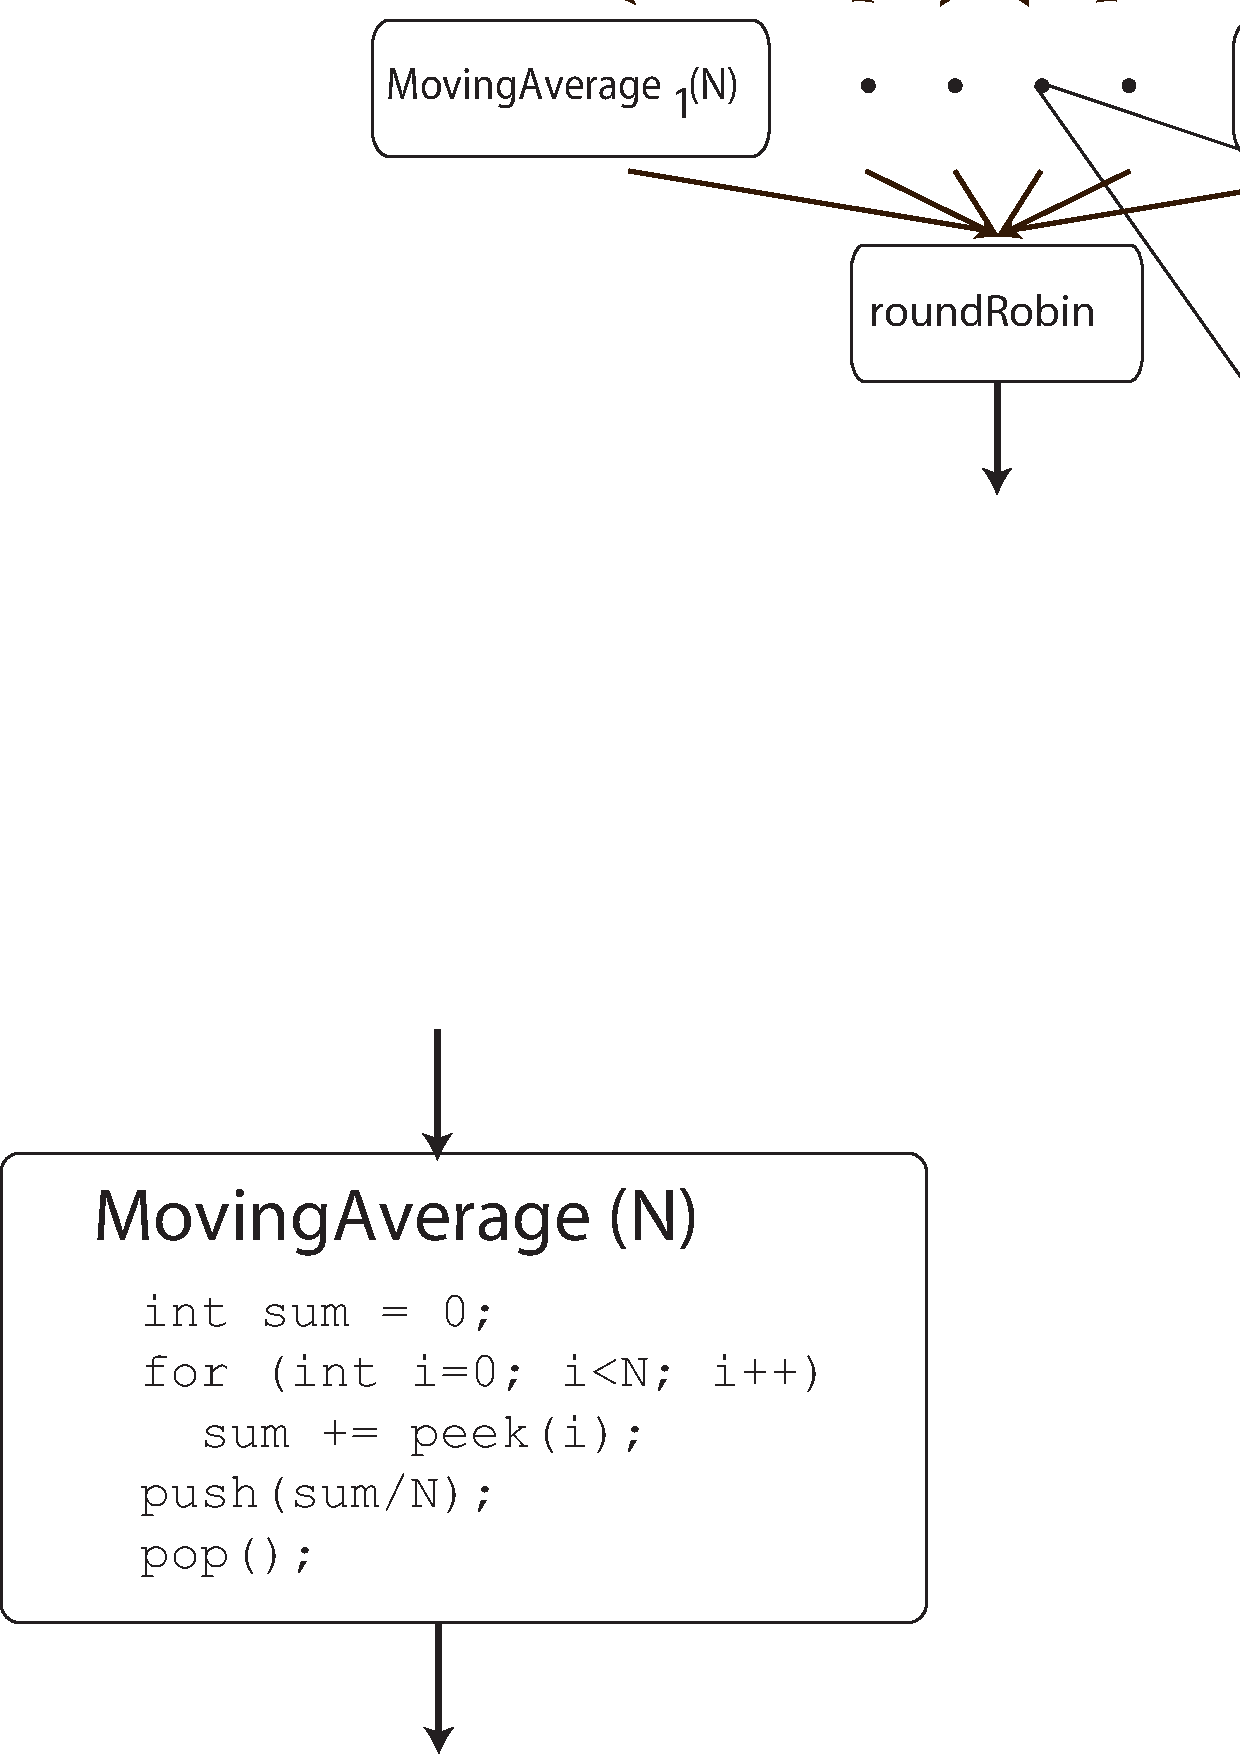
\includegraphics[width=3.4in]{figures/duplicate-fission.pdf}
\caption{Fission of a filter that peeks. \protect\label{fig:duplicate-fission-example}}
\end{figure}


\begin{figure*}[t!]
\centering
\includegraphics[width=6.5in]{figures/fission-example.pdf}
\caption{Example of an iteration filter fissed into three fission products each with multiplicity 2.  The chart indicates the values used to determine the next value of the iteration field.  
\protect\label{fig:fission-example}}
\end{figure*}

The compiler introduces data parallelism to the streaming program through a process known as {\it fission}.  Fission is the process of duplicating the stateless filter and wrapping these duplicates in a round-robin splitter and joiner.  The process ensures that input data is distributed correctly and output data is collected in correct order.  The duplicated filters, known as products, can be assigned to individual cores, thus introducing data parallelism.  

Graphically, fission yields a stream graph result as depicted in Figure~\ref{fig:duplicate-fission-example}.  The base filter, MovingAverage, is duplicated into a duplicate splitjoin and joined in a roundrobin fashion.  Each individual MovingAverage$_j$ product has the work function of the base filter with additional bookkeeping measures to maintain the consistency of the channel inputs and outputs.

Fission is applicable only to stateless filters, as the duplication process does not guarantee consistent behavior if filters contain state that changes between iterations.  Because the desugared iteration filters actually use mutable state to keep track of iteration values, the fission process must be modified to handle iteration values.  

\subsubsection{Modifications to Fission Process}

Let $F$ be the stateless filter that will be fissed.  Assume the fission process yields $N$ fissed products.  Accordingly, this yields the fissed products $F_0$, $F_1$, ... , $F_i$, ... , $F_{N-1}$.  The notation $F_{i}$ represents the $(i+1)$th fissed product of filter $F$.

The fission process now modifies the fission products by adding the
following values as fields to the products:
\begin{itemize}
    \item \texttt{init}: the multiplicity of the initialization schedule.  This value is determined for $F$ and is constant for all fissed products.
    \item $\texttt{reps}_i$: how often the \texttt{work} function of the product $F_i$ is
      invoked between rounds.
    \item $\texttt{start}_i$: the value of the induction variable each product $F_i$ starts with, less the initialization multiplicity.  Alternatively, $\sum_{j=0}^{i-1}{\tt reps}_j$ of all fission products preceding the current product.
    \item \texttt{total}: the periodic multiplicity of $F$.  Alternatively $\sum_{j=0}^{N-1}{\tt reps}_j$. This value is the same for all fissed products.
\end{itemize}
As described in ~\ref{sec:compiler-overview}, initialization execution is required for peeking filters to ensure every firing of the periodic steady-state schedule maintains the same number of leftover items on the channel.  This initialization execution of the original filter is transferred entirely to the first fission product.  However, all fission products must take the multiplicity of the initialization schedule into account in their calculations as the multiplicity is adjusted upwards by this value.

Accordingly, the fission product $F_i$ should start each round with iteration values of
\begin{eqnarray*}
\texttt{total}*\texttt{k} + (\texttt{start}_i + \texttt{init})
\end{eqnarray*}
and range up to the value
\begin{eqnarray*}
\texttt{total}*\texttt{k} + (\texttt{start}_i + \texttt{init}) + \texttt{reps}_i - 1
\end{eqnarray*}
where \texttt{k} is a nonnegative integer indicating how many rounds have
been run in the span of the program.  

At the end of each fission product's \texttt{work}, a check must be made to see if it is necessary to increment the induction variable to the next round of values.  This will prevent certain fissed products from making calls with duplicate iteration values.  This check is done after the field incrementing statement.
\begin{eqnarray*}
(\texttt{iter}_{i,k} - (\texttt{start}_i + \texttt{init}) - \texttt{reps}_i) \% \texttt{total} &==& 0
\end{eqnarray*}
This is consistent with the maximum value per round as
indicated above.  Only when we reach this maximum value does subtracting 
$\texttt{start}_i$, \texttt{init}, and $\texttt{reps}_i$ from $\texttt{iter}_i$ leave a value divisible by
\texttt{total}.

Once the fissed product's iteration value has reached
this value, it must be set to:
\begin{eqnarray*}
\texttt{iter}_{i,k+1} &=& \texttt{iter}_{i,k} + (\texttt{total} - \texttt{reps}_i) \\
&=& \texttt{total}*\texttt{k} + (\texttt{start}_i + \texttt{init}) + \texttt{reps}_i \\
&&  \ \ +\ (\texttt{total} - \texttt{reps}_i) \\
&=& \texttt{total}*(\texttt{k+1}) + (\texttt{start}_i + \texttt{init})
\end{eqnarray*}
which is the starting iteration value of the next round, as defined.

\subsubsection{Accounting for Steady-state Schedule Modification}

Other passes may modify the steady-state schedule after fission, increasing the multiplicity of the fission products.  This scales the $\texttt{reps}_i$ field for all products.  $\texttt{start}_i$ and $\texttt{total}$ are dependent on $\texttt{reps}_i$ and must be scaled accordingly.

Assume a pass increases hte steady-state multiplicity of our filter to $m$.  We expect the fission product $F_i$ to start round $k$ with iteration values of 
\begin{eqnarray*}
(\texttt{total}*\texttt{k}*m) + (\texttt{start}_i*m + \texttt{init})
\end{eqnarray*}
The filter should perform $\texttt{reps}_i$*$m$ iterations, thus should range up to value
\begin{eqnarray*}
(\texttt{total}*\texttt{k}*m) + (\texttt{start}_i*m + \texttt{init}) + (\texttt{reps}_i*m) - 1
\end{eqnarray*}

Between rounds, iteration values must be incremented by the actual total number of repetitions that occur.  All fission products perform a total of $\sum(\texttt{reps}_{i}*m)$ repetitions which is simply \texttt{total}*$m$.  Thus, the updating step will still hold:
\begin{eqnarray*}
\texttt{iter}_{i,k+1} &=& \texttt{iter}_{i,k} + (\texttt{total}*m - \texttt{reps}_i*m) \\
&=& \texttt{total}*\texttt{k}*m + (\texttt{start}_i*m + \texttt{init}) + \texttt{reps}_i*m \\
&&  \ \ +\ (\texttt{total}*m - \texttt{reps}_i*m) \\
&=& \texttt{total}*(\texttt{k+1})*m + (\texttt{start}_i*m + \texttt{init})
\end{eqnarray*}

Figure~\ref{fig:fission-example} shows the filter from Figure~\ref{fig:desugar} fissed into three fission products, each with multiplicity 2.  The accompanying charts for each fissed product are as follows:
\begin{itemize}
\item{\tt iter} indicates the value of the {\tt iter} field at the start of the filter invocation.  
\item{\tt iter++} indicates the value of the {\tt iter} field incremented by 1 (which is the value {\tt iter} takes prior to the check.  
\item{\tt check} indicates the value of $(\texttt{iter}_{i,k} - (\texttt{start}_i + \texttt{init}) - \texttt{reps}_i)$, which must be divisible by {\tt total} in order to advance to the next round.  
\item{\tt next} indicates the value {\tt iter} will take at the next invocation of the fissed product.
\end{itemize}
Note that the value of \texttt{iter} jumps to the next round of values with multiplicity 2, as expected.
%\section{Data Parallelization Common Case}

% The techniques covered above are employed during the compiler flow
% outlined in Chapter~\ref{ch:datapar} to effectively leverage data and
% task parallelism.  The coarsened StreamIt graph is converted into a
% general by employing \textsc{SynchRemove} (see
% Section~\ref{sec:synch-remove} for details).  \textsc{JudiciousFission} is
% performed on the coarsened general graph using the technique covered
% in Section~\ref{sec:levels}.  Fission of a node in the general graph
% replaces fission of a filter in the StreamIt graph (see
% Section~\ref{sec:fission-streamit}) in the process of judicious
% fission.  Conversion to the general graph with synchronization
% removal, accompanied by employing general fission, greatly reduces the
% inter-core communication requirement of the resulting mapping when
% fissing filters that peek.  Figure~\ref{fig:fission-versus} gives a
% simple example of the potential savings.

% The design of the general fission algorithm was informed by the fact
% that for most fission applications of judicious fission, a producer
% and consumer are fissed by an equal width.  This is because in most of
% our benchmarks, a level's width of task parallelism is equal to the
% width of task parallelism for it's consuming level.  In this case,
% fission on the general graph will map the bulk of communication to
% intra-core resources.  Furthermore, in the next section we demonstrate
% that the ratio of inter-core communication to total communication is
% parametrizable for this case.

To understand why general fission achieves the reduction of inter-core
communication for this case, we must remember a few properties of the
steady-state schedule of the stream graph.  For single output producer
$f$ and single input consumer $g$, where $(f,g) \in E$:

\[ M(S, f) \cdot u(W, f) = M(S,g) \cdot o(W,g) \]

\noindent When $f$ and $g$ are fissed (employing general fission) by
the same amount $P$, the above equality no longer holds across all the
fission products if $g$ peeks.  This is because the peeking of $g$ is
converted into duplication of items to the products of $g$'s fission
application.  The fission products of $g$ each consumes more items
than each fission product of $f$ produces.  However, we can make it
the case that {\it most} of the outputs of a fission product $f_i$ are
directed to $g_i$, for each $1 \le i \le P$.  When each $f_i$ and
$g_i$ are mapped to the same core, the bulk of communication is
intra-core.

\begin{figure*}[t]
\centering
\includegraphics[width=6in]{figures/core-comm.pdf}
\caption[Communication between cores for fission of producer and
consumer.]{ Communication details for fission products of consumer $f$
  and producer $g$ each fissed by $P$.  $f$ was a single output node,
  and $g$ was a single input node.  Furthermore, $C(g) = \mt{dup}_g$.
  Each $f_i$, $g_i$ pair are mapped to the same core.
  The sizes of the buffer sections are in terms of $g$. Red arrows
  denote inter-core communication. \label{fig:core-comm}}
\end{figure*}

Figure~\ref{fig:core-comm} illustrates the details of communication
between $f$ and $g$ when each is fissed by $P$.  In the figure it is
assumed that $C(g) = \mt{dup}_g $, meaning the number of items
remaining after the initialization schedule equals the number of items
that $g$ inspected but did not pop.  Each $f_i$ produces $M(S,f)/p
\cdot u(S,f)$ items, while each $g_i$ must consume the original pop
rate multiplied by it's slice of $f$'s multiplicity plus the number of
inspected items of $g$:

\[ M(S,g)/P \cdot o(W, g) + C(g) \]

\noindent Since $M(S,g)/P \cdot o(W, g) = M(S,f)/p
\cdot u(S,f)$, the number of items each $f_i$ produces and the number
of items each $g_i$ consumes differs by $C(g)$.
As Figure~\ref{fig:core-comm} demonstrates, each $g_i$
receives $C(g)$ duplicated items from $g_{i-1}$ (with $g_1$
receiving from $f_p$).  When the fission products are assigned to
cores as given in the figure, the percentage of inter-core
communication to total communication can be reduced to:

\begin{equation}
\label{eq:min-dup}
\mt{InterCore}(g) = \frac{C(g)}{M(S,g) / P * o(W, g)}
\end{equation}

\noindent This percentage corresponds to the best case, in which a
producer and consume are fissed by the same amount and $C(g) =
\mt{dup}_g$.  This case is common in our benchmarks.

The next section covers a technique that seeks to decrease the percentage
of total communication that must be communicated inter-core.  The
technique directly decreases the number of items that are shared,
while also increasing the alignment of communication to minimize
inter-core communication.

\section{Sharing Reduction}

A key design goal for the implementation of fission was that
communication between producers and consumers of the stream graph be
efficient.  Often when data parallelism is applied, the producer
filter is fissed by the same factor as the consumer filter.  To make
this common case efficient, general graph fission communicates a large
number of items between disjoint producer-consumer pairs of products
of the fission.  Next, a small number of items (the number of items
inspected by the consumer filter) is duplicated and communicated from
producer to a consumer in a different pair.

\begin{figure*}[t]
\centering
\includegraphics[width=6in]{figures/remaining-dup-case.pdf}
\caption[Extra inter-core communication when $C(g) > \mt{dup}_g$.]
{Inter-core communication details for fission products of consumer $f$
  and producer $g$ each fissed by $P$.  $f$ was a single output node,
  and $g$ was a single input node.  For $g$, $C(g) > \mt{dup}_g$.
  Each $f_i$, $g_i$ pair are mapped to the same core.  The sizes of
  the buffer sections are in terms of $g$. Red arrows denote
  inter-core communication.  \label{fig:remaining-dup}}
\end{figure*}

Figure~\ref{fig:remaining-dup} illustrates the details of
communication between $f$ and $g$ when each is fissed by $P$ with each
$f_i$ mapped to a distinct core, and to the same core as $g_i$.  From
the figure, notice that $C(g)$ items are communicated from $f_i$ to
$g_{i+ 1}$, with $f_P$ sending to $g_1$.  Of the $C(g)$ items,
$\mt{dup}_g$ items are required by both $g_i$ and $g_{i+1}$.  This
corresponds to the orignal number of input items of $g$ that were
inspected by not dequeued for one firing of $g$.  The remaining items,
$C(g) - \mt{dup}_g$, are required to be transfered from $f_i$ to
$g_{i+1}$ when $C(g) > \mt{dup}$ because of misalignment of the items
produced by $f_i$ and required by $g_i$.

When the fission products are assigned to
cores as given in the figure, the percentage of inter-core
communication to total communication can be quantified as:

\begin{equation}
%b\vspace{-2pt}
\label{eq:min-dup}
\mt{InterCore}(g) = \frac{C(g)}{M(S,g) / P * o(W, g)}
%\vspace{-4pt}
\end{equation}

\noindent This percentage corresponds to inter-core communication
ratio for each product filter and, since all product filters have the
same rates, for the total inter-core communication required for the
fission of $g$.

This section covers a technique that seeks to decrease the percentage
of total communication that must be communicated inter-core.  The
technique directly decreases the number of items that are shared,
while also increasing the alignment of communication to minimize
inter-core communication.

Since streaming applications typically execute for many iterations of
the steady-state, it is legal to increase the steady state by $c$.  As
long as this constant $c$ is less than the number of steady-state
iterations $I$ of the application, and $c$ is a factor of $I$.

By recognizing this property, we can directly reduce the amount of
inter-core communication that occurs between the fission products of a
fissed peeking filter for many cases of general fission, including the
common case.  In Equation~\ref{eq:min-dup} we can directly control the
steady-state multiplicity of $g$, $M(S,g)$.  We can calculate a
constant $c_g$ such that the percentage is less than a threshold
$T_{\mt{sharing}}$:

\begin{equation}
\label{eq:ic-thresh}
c_g = \frac{1}{T_{\mt{sharing}}} \cdot \frac{C(g) \cdot P}{M(S,g) \cdot o(W,g)}
\end{equation}

\noindent where $0.0 < T_{\mt{sharing}} \le
\mt{InterCore(g)}$. Increasing the steady-state of the graph by $c_g$
before general fission is applied will assure that the percentage of
items duplicated will be equal to $T_{\mt{sharing}}$.  Sharing
reduction works by increasing the ratio of number of items that are
only needed by one product to the number of items that are needed by
two products.  When we increase the steady-state, in
Figure~\ref{fig:remaining-dup}, the shared (red) sections of the input
buffer to $g$ remain fixed in size, while the private sections of the
input buffer (black) grow.

\subsection{Sharing Reduction for Other Fission Cases}

The sharing reduction optimization does not apply as simply to all
cases of fission of a peeking filter.  Consider the case where we have
single output producer $f$ and single input consumer $g$ with $(f,g)
\in E$, but $f$ and $g$ are fissed by differing widths, i.e., $P_f \ne
P_g$.  This case engenders inter-core communication not only because
of sharing but because of the communication required by the differing
fission widths.  

Going forward, let us assume that $P_f > P_g$.  If $P_f$ is a multiple
of $P_g$, the analysis is straightforward: the percentage of
inter-core communication to total communication is $(1 -
\frac{P_g}{P_f}$). If $P_f$ is not a multiple of $P_g$ misalignment
also occurs because for one or more $g_j$, it's input does not begin
in alignment with any $f_i$'s.  The analysis of the percent of
inter-core communication for this latter case is complex, but it
suffices for our purposes to bound it by $(1 - \frac{P_g}{P_f})$.

Also consider the case where $g$ has multiple inputs. In this case $g$
receives $\mt{RI}(f, g, S) \cdot M(S, g) \cdot o(W,g)$ items from $f$
during the steady-state, and $(1 -\mt{RI}(f, g, S) \cdot M(S, g) \cdot
o(W,g))$ from its other producers. There is a choice: for which
producer of $g$ to optimize the communication of $g$? If $f$ is
chosen, then the assignment of filters to cores should minimize the
inter-core communication by co-locating the fission products of $f$
and $g$ just as the assignment would when $g$ is single input.
However, the calculation must now account for the inter-core
communication of the other producers sending to the fission products
of $g$. 

Now, considering both cases above, we define $\mt{InterCore}(g, f)$ to
approximate the percentage of inter-core communication to total
communication for the input of the fission products of $g$ optimizing
for the placement of the fission products of $f$:

\begin{equation}
\label{eq:tcomm-fopt}
 \mt{InterCore}(g, f)   =  (1 -\mt{RI}(f,g, S) \cdot \frac{P_g}{P_f})
 + \frac{P_g \cdot C(g)}{M(S, g) \cdot o(W, g)}
\end{equation}

\noindent The first term approximates the inter-core communication due
to (i) the fission factor discrepancy between $f$ and $g$, and (ii) the
multiple inputs of $g$.  The second term quantifies the percentage of
inter-core communication caused by the sharing due to peeking.

Increasing the steady-state will not alter the first term of
Eq.~\ref{eq:tcomm-fopt}.  However, the second term can be reduced
because a smaller percentage of steady-state items needs to be
duplicated.  By Amdahl's law, increasing the steady-state can only
decrease $\mt{InterCore}(g, f)$ to under $T_{\mt{sharing}}$ if the
second term of Equation~\ref{eq:tcomm-fopt} accounts for more than
$(1-T_{\mt{sharing}} )$ of the duplication.  

We need to prevent the application of increasing the steady-state to a
filter $g$ that will not benefit from it because the majority of
inter-core communication from fission of $g$ is not caused by $g$'s
sliding window.  We define a constant $T_{\mt{apply}}$ such that
sharing reduction should only be applied to $g$ optimizing for $f$ if:

\begin{equation}
\label{eq:apply-sharing}
T_{\mt{sharing}}  >  T_{\mt{apply}} \ge (1 -\mt{RI}(f,g, S) \cdot
\min(\frac{P_g}{P_f}, \frac{P_f}{P_g}))
\end{equation}

% \begin{equation}
% T_{\mt{sharing}}  >  T_{\mt{apply}} \ge (1 -\mt{RI}(f,g, S) \cdot
% \frac{P_g}{P_f})
% \end{equation}

\noindent Since it was first assumed that $P_f > P_g$, in order to
generalize we must choose the appropriate fraction of local
communication by taking the minimum of the two fission width ratios.

In the common case where $f$ and $g$ are fissed by the same width, and
$f$ has single output and $g$ has single input, the RHS of
Eq.~\ref{eq:apply-sharing} evaluates to 0, indicating to always apply
sharing reduction.  If however, the RHS of Eq.~\ref{eq:apply-sharing}
does not evaluate to 0, there exists inter-core communication that is
not attributed to sliding windows.  In this latter case,
$T_{\mt{apply}}$ determines at what percent of total inter-core
communication, non-sliding-window inter-core communication should
prevent the application of sharing reduction.  For example, if
$T_{\mt{apply}} = .05$, then we will apply sharing reduction only when
sliding window inter-core communication accounts or at least 95\% of
total inter-core communication for the proposed fission application of
$g$. $T_{\mt{apply}}$ prevents the application of sharing reduction to
fission when the bulk of inter-core communication of the fission is
not caused by sliding windows, and thus will not be reduced by
increasing the steady-state.

% For simplicity of analysis, let us assume that $C(g)
% = 0$, and $P_f$ is a multiple of $P_g$. Figure~\ref{fig:diff-widths}
% presents an example with these assumptions.  In the example, $f$ and
% $g$ are fissed by 8 and 4 respectively.  Since we want to maintain
% data parallelism, each $f_i$, $1 \le i \le P_f$, is mapped to a
% distinct core, as is each $g_j$, $1 \le j \le P_g$.  Since each $f_i$
% produces half the number of items required by each $g_j$, half the
% communication in this case is inter-core, caused by the misalignment
% of the rates of the producer and consumer fission products.


% Additionally, if $C(g) > 0$, it is required to share $C(g)$ items
% between two cores.  There are $P_g$ sections of $C(g)$ items, and this
% data has to be communicated inter-core to one other core.  Given this
% analysis, we can quantify an {\it approximation} of the percentage of
% inter-core communication for the fission application of $g$ when $P_f
% > P_g$:

% \begin{align}
% \mt{InterCore}(g) & = & \frac{(1 - \frac{P_g}{P_f}) \cdot M(S, g) \cdot o(W, g) +
% P_g \cdot C(g)}{M(S, g) \cdot o(W, g)} \\
% \label{eq:diff-fiss}
% \mt{InterCore}(g) & = & (1 - \frac{P_g}{P_f}) +
% \frac{P_g \cdot C(g)}{M(S, g) \cdot o(W, g)}
% \end{align}

% The first term on the RHS of Equation~\ref{eq:diff-fiss} gives the
% percentage of inter-core communication produced by the fission width
% inequality.  

% \begin{equation}
% \label{eq:tcomm-fopt1}
%  \mt{InterCore}(g,f)   = (1 - \mt{RI}(f,
%    g, S))  + (1 - \frac{P_g}{P_f}) \cdot \mt{RI}(f,
%    g, S)   + \frac{P_g \cdot C(g)}{M(S, g) \cdot o(W, g)} 
% \end{equation}

% \noindent The first term accounts for the percentage of items that $g$'s fission
% products receive from producers that are not products of $f$.  The
% second term, the percentage items that are communicated inter-core
% because of the fission width mis-alignment, must now account for the
% fact that not all items are from $f$.  Equation~\ref{eq:tcomm-fopt1}
% can be simplified to:


\subsection{Sharing Reduction Applied to the Stream Graph}
So far we have considered the application of the sharing reduction
optimization to a single filter $g$ in the stream graph.  Now we will
cover how to apply sharing reduction across all the filters of the
stream graph for which it is appropriate.  The goal is reduce the
percentage of inter-core communication due to the sharing between
fission products of all peeking filters to {\it approximately}
$T_{\mt{sharing}}$ of total inter-core communication for the fission
of all peeking filters.  Sharing reduction may not achieve
$T_{\mt{sharing}}$ because there may exist peeking filters that are to
be fissed for which Equation~\ref{eq:apply-sharing} cannot be
satisfied.  For these filters, we do not apply the sharing reduction
optimization.

The process of applying sharing reduction to the entire stream graph
consists of determining which filters are appropriate and determining
a steady-state multiplier by which to increase the graph.  To
determine the steady-state graph multiplier, the compiler calculates
the percentage of sharing over all of the filters which adhere to
Equation~\ref{eq:apply-sharing}.  Let $\Phi$ denote the set of filters
for which Equation~\ref{eq:apply-sharing} holds and that we seek to
fiss:

\begin{equation}
\label{eq:sr-mult}
c = \frac{1}{T_{\mt{sharing}}} \cdot \frac{\sum_{g \in \Phi} P_g \cdot C(g) }{\sum _{g \in
    \Phi} M(S, g) \cdot o(W, g)}
\end{equation}

\noindent Increasing the steady-state by $c$ for all filters of the
graph will reduce the total sharing for the filters of $\Phi$ to
$T_{\mt{sharing}}$.  




% In the
%  graph before fission is applied, $C(g)$ items will remain in the
%  input buffer of $g$ between steady-state iterations.  After fission by $P$,
%  for each steady-state, $g_1$ will first consume the $C(g)$ items that
%  $f_p$ sent it from the previous steady-state iteration.  $g_1$ will
%  then require:

% \[ M(S, g)/P \cdot o(W, g) + \mt{dup} - C(g)\]

% \noindent additional items from $f_1$.\footnote{It is guaranteed that
%   $M(S, g)/P \cdot o(W, g) > C(g)$ by the precondition of general
%   fission.} This requirement is less than the number of items that
% $f_1$ produces $M(S, g)/P \cdot o(W, g)$ since $C(g) > \mt{dup}$. So,
% $C(g) - \mt{dup}$ items must be transferred from $f_1$ to $g_2$ in
% addition to the shared and duplicated $\mt{dup}$. In all, $C(g)$ items
% must be transferred from $f_i$ to $g_{i+1}$.

%  Each $f_i$ produces $M(S,f)/p
% \cdot u(S,f)$ items, while each $g_i$ must consume the original pop
% rate multiplied by it's slice of $f$'s multiplicity plus the number of
% inspected items of $g$:

% \[ M(S,g)/P \cdot o(W, g) + C(g) \]

% \noindent Since $M(S,g)/P \cdot o(W, g) = M(S,f)/p
% \cdot u(S,f)$, the number of items each $f_i$ produces and the number
% of items each $g_i$ consumes differs by $C(g)$.
% As Figure~\ref{fig:core-comm} demonstrates, each $g_i$
% receives $C(g)$ duplicated items from $g_{i-1}$ (with $g_1$
% receiving from $f_p$).  

\section{Data Parallelization of Stream Graph}
\label{sec:data-par}

The techniques in this paper are employed by the parallelization
management phase of the compiler once the width of
data-parallelization for each filter is calculated.  Previous work
describes numerous effective techniques for managing the
parallelization of a stream
graph~\cite{kudlur08,gordon-asplos06,flextream,udupa09-gpu,liao06brook}.
Note that our framework extends to cyclic graphs as along as there is
enough delay in any backedge to account for the increase in the
steady-state multiplicity factor that is applied by our techniques.
In StreamIt, for example, this delay can be specified using the
{\tt enqueue} block.

\textsc{DataPar} of Algorithm~\ref{alg:data-parallelize} presents an
algorithm for applying fission of sliding window filters with sharing
reduction across the entire stream graph.  The extent of data
parallelism for each filter is decided by the parallelization
management phase, and is an argument to our algorithm, $P=(V
\rightarrow \mathbb{N})$. 

The compiler is required to calculate a multiplication factor $c$ for
the entire graph that satisfies the preconditions for fission for
every filter that will be fissed (see Section~\ref{sec:fission}).  At
the same time, $c$ applies sharing reduction to these filters by
increasing the steady-state such that Equation~\ref{eq:sr-mult} is
satisfied by the constant.

\begin{algorithm}[t]
\caption{Exploit Data Parallelism in $G$ for $N$
  Cores} \label {alg:data-parallelize}
\footnotesize
\textsc{DataPar}($G=(V, E), N, T_{\mt{sharing}},
T_{\mt{apply}}, P=(V \rightarrow \mathbb{N}) $)
\begin{algorithmic}[1]
\State $\mt{preCondMult} \gets 1$, $\mt{sharingItems} \gets 0$, $\mt{totalItems} \gets 0$
\State $\triangleright$ Calculate multiplier for fission preconditions and sharing reduction
\ForAll {$g \in V$}
\State $\triangleright$ If this is a peeking filter we are fissing:
\If {$P_g > 1 \wedge C(g) > 0$}
\State $\triangleright$ Find the producer of $g$ with the lowest
value for Eq.~\ref{eq:apply-sharing}
\State $f \gets \min_{f \in \mt{In}(g)} (1 -\mt{RI}(f,g, S) \cdot
\min(\frac{P_g}{P_f},\frac{P_f}{P_g} )) $
\label{ln:dp1}
\State $\triangleright$ If Eq.~\ref{eq:apply-sharing},
then record the sharing and total communication
\If {$T_{\mt{apply}} \ge  (1 -\mt{RI}(f,g, S) \cdot
\min(\frac{P_g}{P_f},\frac{P_f}{P_g} ))$}
\State $\mt{sharingItems} \gets \mt{sharingItems} + P_g \cdot C(g)$
\State $\mt{totalItems} \gets \mt{totalItems} + M(S,g) \cdot o(W, g)$
\EndIf 
\State $\triangleright$ Assure that fissing peeking filters adhere to Eq.~\ref{eq:fiss-precond1}
\State $\mt{preCondMult} \gets \max(\mt{preContMult}, \frac{C(g) \cdot P_g}{M(S,g)
 \cdot o(W,g)})$  
\label{ln:dp3}
\EndIf
\EndFor
%\Statex
\State $\triangleright$ Find the multiplier for sharing reduction
\State $\mt{minMult} \gets T_{\mt{sharing}} \cdot \frac{\mt{sharingItems}
}{\mt{totalItems}}$
\label{ln:dp2}
\State $\triangleright$ Make sure multiplier assures all fissing peeking filters
adhere to  Eq.~\ref{eq:fiss-precond1}
\State $\mt{minMult} \gets \max(\mt{minMult}, \mt{preCondMult})$
\State $\triangleright$ Find the LCM of the $P_f$'s
greater than $\mt{minMult}$ to adhere to Eq.~\ref{eq:mod-fiss}
\State $c \gets $\Call{LCM}{$\forall P_f | f \in V$} $ >
\mt{minMult}$
%\Statex
\label{ln:dp4}
\State $\triangleright$ Increase the steady-state by $c$
\ForAll {$f \in V$}
\State $M(S,f) \gets c \cdot M(S, f)$
\EndFor
%\Statex
\State $\triangleright$ Apply general fission to all nodes in the graph
\ForAll {$f \in V$}
\State \Call{GeneralFiss}{$f$, $P_f$}
\EndFor
\end{algorithmic}
\end{algorithm}

For each peeking filter $g$ that will be fissed, line~\ref{ln:dp1}
finds the producer of $g$ that minimizes
Equation~\ref{eq:apply-sharing}.  If this value is below
$T_{\mt{apply}}$, $g$ is added to the sharing reduction calculation by
adding $g$'s shared items and $g$'s total items to the running totals
of each quantity.  Sharing reduction is incorporated into the
steady-state multiplier $\mt{minMult}$ in line~\ref{ln:dp2} employing
Equation~\ref{eq:sr-mult}.  The algorithm applies
Equation~\ref{eq:fiss-precond1} to each peeking filter that will be
fissed by maintaining a running value of the minimum multiplier that
enforce the precondition (line~\ref{ln:dp3}).  The sharing reduction
multiplicity ($\mt{minMult}$) is required to be greater than the
precondition multiplier.  Because of the precondition of
Equation~\ref{eq:mod-fiss}, the final multiplication factor for
increasing the steady-state must be a multiple of all the fission
widths of the map $P$. The algorithm assures this by finding the least
common multiple of all the $P_f$'s greater than $\mt{minMult}$
(line~\ref{ln:dp4}).  The steady-state multiplicity of the graph is
then increased by $c$.  Finally, each filter $f$ can be fissed by $P_f$
using the fission transformation of Section~\ref{sec:fission}.




\section{Results}
\label{chpt:results}

This section presents results of creating schedules using
techniques described in Sections \ref{chpt:hierarchical} and
\ref{chpt:phased}.

Section \ref{sec:results:apps} presents the applications used for
testing.  Section \ref{sec:results:results} presents the results and
analysis.

\subsection{Applications}
\label{sec:results:apps}

Our benchmark suite contains 17 applications. Out of those
applications, 15 represent useful practical computation taken from
real-life applications, while two were chosen to highlight the
effectiveness of phased scheduling.

SJPeek1024 and SJPeek31 are synthetic benchmarks, designed to
highlight strengths of phased schedules. SJPeek1024 requires an
initialization schedule which benefits from finer granularity of
minimum latency schedule. SJPeek31 contains a push/pop mismatch
which causes a combinatorial blow-up using SAS.

Nine test applications (BitonicSort, FFT, FilterBank, FIR, Radio,
GSM, 3GPP, Radar and Vocoder) are applications used in
\cite{Gordo02}. BitonicSort performs a 32 element bitonic sort.
FFT performs a 64-element FFT, FilterBank is an 8 channel filter
bank.  FIR is a 64-tap FIR application. Radio is an FM radio
decoder with an equalizer.  3GPP is a 3GPP Radio Access Protocol
application. Radar is a radar array front-end application. Vocoder
is a 28 channel Vocoder.

Two test applications (QMF and CD-DAT) are applications used in
another publication on scheduling streaming applications
(\cite{murthy99buffer}). QMF is a filter bank application. CD-DAT
is a sample rate conversion application. The code inside of the
{\filters} has not been implemented. QMF application is a
qmf12\_3d.  It was slightly modified to account for {\StreamIt}
{\splitters} and {\joiners} not allowing any computation. The
high-pass and low-pass filtering in the {\splitters} has been
moved to just after data has been separated into two channels. The
re-combining of data in the {\joiners} has been moved to a
{\filter} just after the {\joiners}. The low and high pass filters
have also been given a peek amount of 16 so they can perform their
function in the way intended in {\StreamIt}.
 CD-DAT is exactly the same application as
that described in \cite{murthy99buffer}.

The remaining 4 applications were chosen from our sample
applications used for testing the StreamIt compiler. HDTV performs
a HDTV signal decoding/encoding. CFAR implements PCA Constant
False Alarm Rate detection. Block Matrix Mult performs a blocked
matrix multiplication application - it multiplies a 12x12 matrix
by a 9x12 matrix in blocks of 3x3 submatrices. Trellis performs
trellis encoding/decoding.

\begin{comment}

\subsection{Methodology}
\label{sec:results:methodology}

The following data has been collected: number of nodes, number of
node executions per steady state, schedule size and buffer size
for pseudo single appearance and minimal latency schedules.

\subsubsection{Schedule Compression}

\end{comment}

\begin{comment}
\subsubsection{Sinks}

Any application in {\StreamIt} must receive its data from outside,
and its data must be sent to outside. {\filters} that receive and
send data to outside are called sinks and sources. In particular,
sinks have the property of having $u_f = 0$ while sources have
$e_f = o_f = 0$. Sinks are problematic for minimal latency
scheduling, because they do not produce any data. Thus any
schedule of a sink operator is a minimal latency schedule. This
leads to the minimal latency schedule of the outer-most
{\pipeline} becoming a single appearance schedule, thus destroying
some of the benefit of using phased scheduling. The technique
used for scheduling {\pipeline} sinks has been discussed in
\cite{karczma-thesis}.

This problem has been alleviated by detecting sinks at the end of
a {\pipeline} and scheduling them in a unique way. Namely, a simple
attempt is made to minimize the amount of storage necessary to
store the phases of the {\pipeline}.

Let the amount of storage necessary to store one data item in
{\Input} {\Channel} to the sink be $x$, the amount of storage necessary
to store a phase be $y$, the sink consume $a$ data per steady
state execution of its parent {\pipeline} and $b$ be the number of
phases of the parent pipeline, then we have that amount of storage
necessary to store the phases and the buffer is
$$ {ax \over b} + by $$ We want to minimize this amount, with $b$
being the variable. We take a derrivative of the above expression,
set it to zero and solve:

\begin{displaymath}
\begin{array}{rcl}
-{ax \over b^2} + y & = & 0 \\
yb^2 & = & ax \\
b & = & \sqrt{ax \over y}
\end{array}
\end{displaymath}

For simplicity, we set $x = y = 1$, thus obtaining that $b =
\sqrt{a}$.

Now, for every phase of the parent {\pipeline} of the sink, the sink
is executed $\sqrt{a}$ times on the first step of scheduling a
phase of the {\pipeline}.
\end{comment}

\subsection{Results}
\label{sec:results:results}

\begin{figure}[t]
\psfig{figure=buffer-graph.eps,width=3.35in}
\caption{Buffer sizes.}
\end{figure}

\begin{figure}[t]
\psfig{figure=code-graph.eps,width=3.35in}
\caption{Code sizes.}
\end{figure}

\begin{figure}[t]
\psfig{figure=total-size-graph.eps,width=3.35in}
\caption{Sum of code size and buffer size.}
\end{figure}

\begin{table*} \centering \small
\begin{tabular}{|c|c|c|c|c|c|c|}
\hline benchmark & \parbox{0.5in}{\centering number of nodes} & \parbox{0.5in}{\centering number of node executions} & \multicolumn{2}{c|}{pseudo single appearance} & \multicolumn{2}{c|}{minimal latency} \\
\cline{4-7} & & & \parbox{0.5in}{\centering schedule size} & \parbox{0.5in}{\centering buffer size} & \parbox{0.5in}{\centering schedule size} & \parbox{0.5in}{\centering buffer size} \\
\hline SJPeek31 & 6 & 12063 & 8 & 19964 & 24 & 874 \\
\hline HDTV & 170 & 390038 & 230 & 550692 & 1190 & 28300 \\
\hline CD-DAT & 6 & 612 & 6 & 1021 & 64 & 72 \\
\hline CFAR & 4 & 193 & 7 & 193 & 9 & 129 \\
\hline SJPeek1024 & 6 & 3081 & 8 & 7168 & 13 & 4864 \\
\hline Block Matrix Mult & 43 & 1956 & 48 & 4212 & 56 & 3132 \\
\hline Vocoder & 117 & 415 & 156 & 1285 & 205 & 1094 \\
\hline Radar & 68 & 161 & 68 & 332 & 68 & 332 \\
\hline BitonicSort & 370 & 468 & 370 & 2112 & 370 & 2112 \\
\hline 3GPP & 94 & 356 & 104 & 986 & 108 & 970 \\
\hline Trellis & 14 & 301 & 14 & 538 & 17 & 499 \\
\hline FIRfine & 132 & 152 & 132 & 1560 & 132 & 1560 \\
\hline FilterBank & 53 & 312 & 95 & 2063 & 116 & 1991 \\
\hline QMF & 65 & 184 & 85 & 1225 & 85 & 1225 \\
\hline Radio & 30 & 43 & 35 & 1351 & 35 & 1351 \\
\hline FFT & 26 & 448 & 26 & 3584 & 26 & 3584 \\
\hline GSM & 47 & 3356 & - & - & 64 & 3900 \\
\hline
\end{tabular}
\caption{Results of running pseudo single appearance and minimal
latency scheduling algorithms on various applications.}
\label{tbl:results}
\end{table*}

\begin{comment}
\begin{figure}
\centering \psfig{figure=kz-1.eps,width=6in} \caption[Buffer
storage space savings of Phased Minimal Latency schedule vs.
Hierarchical schedule.]{Buffer storage space savings of Phased
Minimal Latency schedule vs. Hierarchical schedule. All data in
all {\Channels} is assume to consume same amount of space.}
\end{figure}

\begin{figure}
\centering \psfig{figure=kz-2.eps,width=6in} \caption[Storage
usage comparison]{Storage usage for compressed Minimal Latency
Phased schedule vs. Hierarchical schedule. Left bars are for
Hierarchical schedules. Numbers are normalized to total storage
required by Hierarchical schedule. Each entry in every schedule
and data items in all {\Channels} are assumed to consume same
amount of space.}
\end{figure}
\end{comment}

Table \ref{tbl:results} presents buffer and schedule sizes
necessary to execute various applications using the algorithms
developed in this thesis.

The GSM application cannot be scheduled using pseudo
single-appearance algorithm, because it has a loop which is too
tight for execution under the SAS.

Several applications show a very large improvement in buffer size
necessary for execution.  Namely, CD-DAT decreases from 1021 to
72, a 93\% improvement. \cite{murthy99buffer} reports a buffer
size of 226 after applying buffer merging techniques. Our
improvement is due to reducing the combinatorial growth of the
buffers using phased scheduling.

Our synthetic benchmarks decrease from 7168 to 4864 and from 19964
to 12063, a 32\% and 40\% improvements. The first improvement is
due to creating fine grained phases which allow the initialization
schedule to transfer smaller amount of data and allow the children
of a {\splitjoin} to drain their data before the {\splitter}
provides them with more. This improvement is only created in
presence of peeking. The second improvement is due to reducing
combinatorial growth and due to finer grained schedules to deal
with peeking.

Other applications show no or little improvement in buffer
requirements. As expected, no application requires more buffer
space.

\mysection{Related Work}
\label{sec:related}

This paper builds directly on the work done to analyze and optimize
linear components in StreamIt graphs \cite{Lamb}. We extend the
theoretical framework for linear analysis to state space analysis in
order to apply our optimizations to a wider class of applications.
Specifically, state space analysis applies to filters with persistent
state, and feedback loops can be combined into a single state space
representation; neither of these cases are handled by linear analysis.
The extension from linear analysis to state space analysis required a
fundamental change to the underlying representation, as well as a
complete reformulation of the rules for combination and expansion.
Moreover, this paper introduces novel optimizations of state removal
and minimal parameterization, both of which operate on the state space
representation.

Several other groups are researching methods for automated DSP
optimizations. SPIRAL \cite{Spiral} is a system developed to generate
libraries of DSP transforms. These libraries are designed for specific
architectures, and can be re-optimized when hardware is upgraded or
replaced. Other such libraries that have been designed include a
package for linear algebra manipulations by the ATLAS project
\cite{Atlas} and portable high-performance FFTs (Fast Fourier
Transforms) \cite{fftw}.

Aside from StreamIt, other programming languages have been designed
for streaming data. Synchronous languages which target embedded
applications include LUSTRE \cite{Lustre}, Esterel \cite{Esterel}, and
Signal \cite{Signal}. Other stream-based languages are Occam
\cite{Occam}, SISAL \cite{sisal}, and StreamC \cite{streamc}.  Some of
these languages are designed to exploit vector and parallel
processing. However, none of these languages have compilers that run
state space or linear analysis.

\section{Conclusion}

This paper shows that the inter-node dependences of a Cyclo-Static
Dataflow Graph can be cleanly represented as a System of Affine
Recurrence Equations.  In combination with Feautrier's array dataflow
analysis~\cite{Feautrier01} for deducing intra-node dependences, this
establishes the SARE as a unified analysis and optimization framework
for high-level DSP programming models.

We believe that the precise affine dependence framework provided by
the SARE representation will enable a powerful suite of node
optimizations in dataflow graphs.  The SARE is a robust and
well-established framework within the systolic and scientific
communities, with methods for graph parameterization, automatic
parallelization, and storage optimization.  We propose optimizations
such as decimation propagation and node fission that are first
applications of these techniques to the signal processing domain.


% \acks
% Acknowledgments, if needed.

% We recommend abbrvnat bibliography style.

\bibliography{references}
\bibliographystyle{abbrvnat}

% The bibliography should be embedded for final submission.

% \begin{thebibliography}{}
% \softraggedright

% \end{thebibliography}

\end{document}
